%!TEX root = ../../../adrien_gomar_phd.tex

\subsection{Static aeroelasticity}
\label{sub:static_aeroelasticity}

Consider a row of a turbomachinery that is in
rotation at a given speed. Due to the centrifugal forces
and the structural and elastic properties of the blade, this
last assumes a deformed position. This is static aeroelasticity.
As the shape of the blade changes, it is not
optimal anymore for the inflow conditions 
and a loss of efficiency is to be expect.
From an engineering standpoint, the problem is thus inverse:
what should be the rigid design of a blade so that under 
loads, the shape is optimum?

When the forces acting on the blade
are too high to achieve a static equilibrium, divergence can occur,
which is a destructive event.
However, according to \citet{Marshall1996}, the stiffness of the
materials used in turbomachinery is large enough to
prevent from static divergence in turbomachines.
This phenomenon will not be studied in this work.

\subsection{Forced response}
\label{sub:forced_response}

As shown previously in Sec.~\ref{sec:cror_unsteady}, wakes and
potentials effects give rise to unsteady fluctuations in 
CROR configurations. These fluctuations 
can generate large vibration levels on the blades,
hence the term forced response. Moreover, as the rotation speed of the
rotors changes within the operating range, the frequency of
the unsteadinesses changes too. If the eigenfrequency
of a blade mode matches the frequency of unsteadinesses or its multiple, 
called Engine Order (EO), resonance can occur. 
This is schematically represented in Fig.~\ref{fig:campbell}
in the so-called Campbell diagram.
Blue points shows the crossing of engine order and 
the blade eigenfrequencies
within the operating range. 
\begin{figure}[htbp]
  \centering
  \includegraphics*[width=0.40\textwidth]{campbell.pdf}
  \caption{Campbell diagram with forced response (blue circles)
  and flutter behavior (red stars).}
  \label{fig:campbell}
\end{figure}

\subsection{Flutter}
\label{sub:flutter}

Flutter is defined as a self-excited, unstable 
self-sustained vibration of a blade in turbomachinery. 
One of the most impressive
manifestation of flutter occurred November 7\textsuperscript{th}, 1940.
Four month after being build, the bridge experienced 
torsional flutter excited by a $64$ \mbox{km/h} wind.
The 1T and 2T modes were observed.
A few hours latter, the bridge felt down as seen in 
Fig.~\ref{fig:tacoma_bridge}. Hopefully, no human
was injured, but this event showed the importance
of taking into account the flutter phenomenon as
it is very energetic and can be a destructive event.
\begin{figure}[htb]
  \centering
  \subfigure[Torsion mode]{
      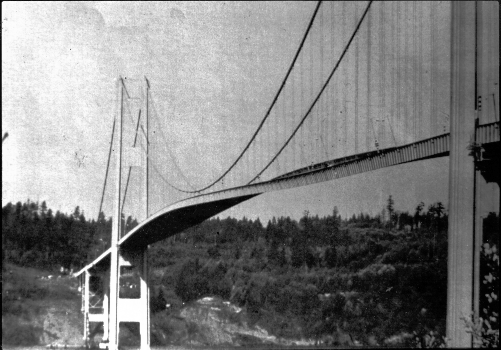
\includegraphics[height=.3\textwidth]{tac06.png}}
  \subfigure[Failure of the bridge]{
      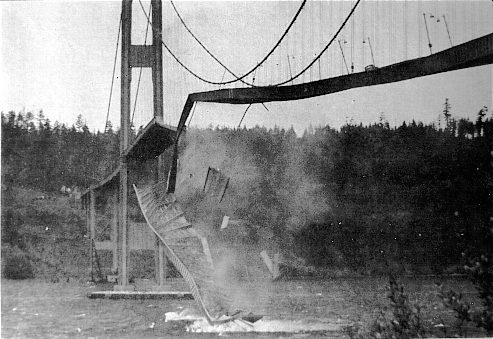
\includegraphics[height=.3\textwidth]{tac09.png}}
  \caption{Tacoma Narrows bridge flutter, from \citet{Smith1974}.}
  \label{fig:tacoma_bridge}
\end{figure}

Three vibration scenarios can appear for flutter.
The first scenario is the damped (or positively damped) 
vibration meaning
that the vibration amplitude decreases with respect to time, 
as shown in Fig.~\ref{fig:flutter_damped}.
This is the most wanted behavior as the system tends to
as stable point. In this case, the blade is said to
be flutter-free.
The second scenario is the amplified (or negatively damped)
vibration as shown in Fig.~\ref{fig:flutter_amplified}. 
This was the scenario that most likely occurred for the
previous example of the Tacoma bridge. This scenario ultimately
leads to failure which is not acceptable. Furthermore, as
detailed in Sec.~\ref{sec:cror_challenges}, the blades of 
a CROR shall not fail otherwise the aircraft might
be destroyed.
The last scenario is the Limit Cycle Oscillation (LCO) vibration.
In this scenario, the deformation increases until a certain 
amplitude and then stays constant. This scenario is not
destructive by essence compared to the amplified scenario. However,
if the blade is repetitively excited by LCO, the blade
can fail as a consequence of the structure fatigue.
\begin{figure}[htb]
  \centering
  \subfigure[damped]{
      \label{fig:flutter_damped}
      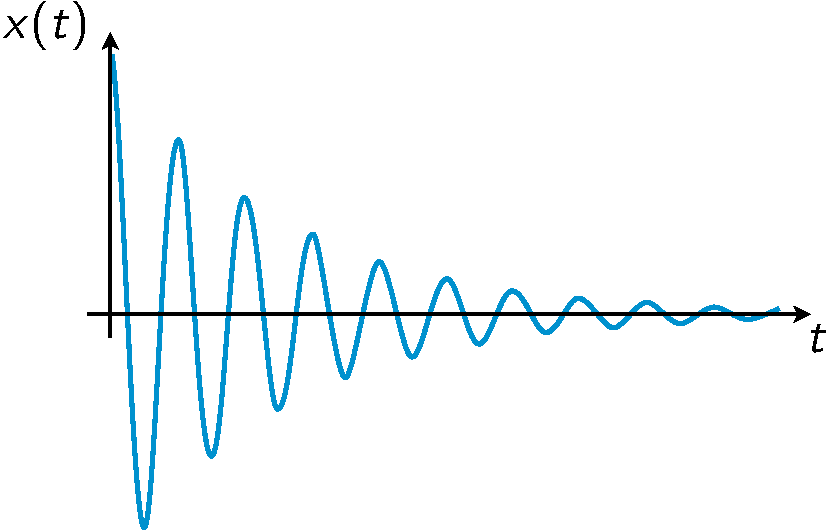
\includegraphics[width=.3\textwidth]{flutter_damped.pdf}}
  \subfigure[amplified]{
      \label{fig:flutter_amplified}
      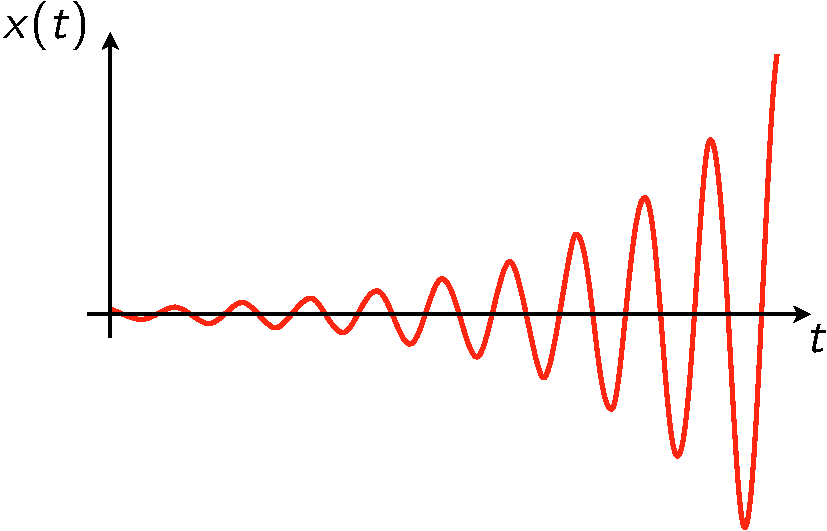
\includegraphics[width=.3\textwidth]{flutter_amplified.pdf}}
  \subfigure[Limit cycle oscillation]{
      \label{fig:LCO}
      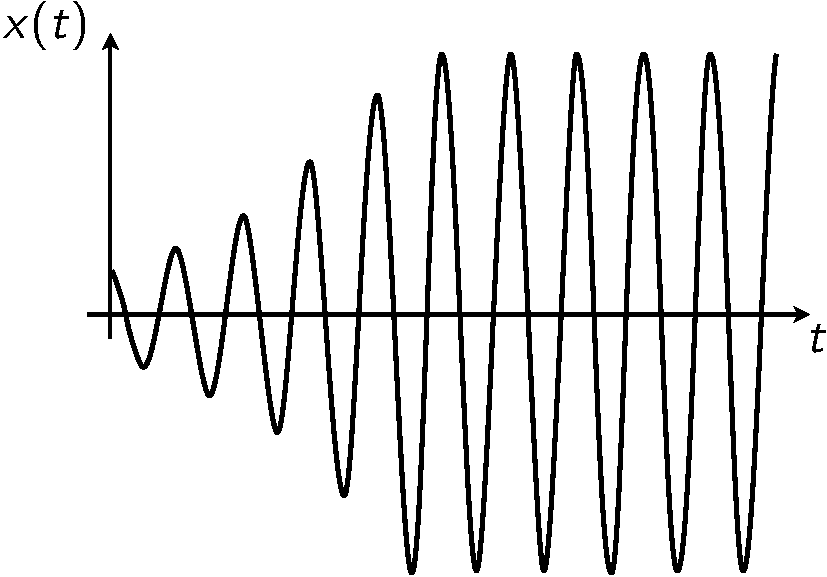
\includegraphics[width=.3\textwidth]{LCO.pdf}}
  \caption{Different vibration scenario for the flutter phenomenon.}
\end{figure}

The development of one scenario over another one is linked to
the fluid response to the vibration of the blade. In fact,
if the aerodynamic loads projected on the direction of the vibration
is positive, this means that the displacement will be amplified. 
In opposite, if the force is in opposed direction, the vibration will be damped.
The out-of-phase component of the aerodynamic force compared to
the displacement vector will give finally the sign of the aerodynamic damping.
The amplitude will give its strength. 
